\section{Materials and Methods}

\subsection{Cognitive Behavioural Therapy (CBT)}
\normalsize{
"Cognitive Behavior Therapy, Second Edition - Basics and Beyond-Judith S. Beck Ph.D. Aaron T. Be" is the primary source for TreadWill's cognitive behavioural therapy (CBT)-based therapeutic content.\cite{beck2011cognitive}
Consequently, it was essential to read the aforementioned work.\\
The basic principles of cognitive behavior therapy are as follows:}
\begin{enumerate}
    \item Cognitive behavior therapy is based on an ever-evolving formulation of patients’ problems and an individual conceptualization of each patient in cognitive terms.
    \item Cognitive behavior therapy requires a sound therapeutic alliance.
    \item Cognitive behavior therapy emphasizes collaboration
and active participation.
    \item Cognitive behavior therapy is goal oriented and problem
focused.
    \item Cognitive behavior therapy initially emphasizes the present.
    \item Cognitive behavior therapy is educative, aims to teach
the patient to be her own therapist, and emphasizes relapse prevention.
    \item Cognitive behavior therapy aims to be time limited.
    \item Cognitive behavior therapy sessions are structured.
    \item Cognitive behavior therapy teaches patients to identify,
evaluate, and respond to their dysfunctional thoughts and beliefs.
    \item Cognitive behavior therapy uses a variety of techniques to change thinking, mood, and behavior. \cite{beck2011cognitive}
\end{enumerate}
\normalsize{
The various TreadWill modules are built on these CBT concepts.
}\\

\subsection{Finite State Machines}
\normalsize{
A finite-state machine (FSM) or finite-state automaton is a computational mathematical model. It is an abstract machine that is always in precisely one of a limited set of states. In response to certain inputs, the FSM may transition from one state to another; this shift is known as a transition.\cite{wang2019formal}\\

It was important to study about finite state machines and create a few prototype FSMs with their state transition diagrams using Python's \textbf{pytransitions} module in order to prepare for future contributions to developing FSM-based modules in the chatbot on TreadWill, WillBot. \\

Before I could understand FSMs, I needed to get familiar with the theory of computing and review the lecture notes from the CS340 class\footnote{Thanks to Prof. Raghunath Tewari}. In order to implement it, I first studied the documentation of the pytansitions module, and then I used Python to implement the examples that were provided. After that, I considered a few real-world applications of FSMs and attempted to develop them in Python along with their state transition diagrams.\\
}

\subsubsection{Turnstile as State Machine}
\begin{figure}[h!]
    \centering
    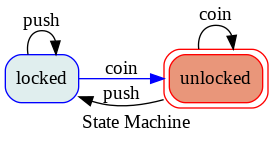
\includegraphics[width=0.4\textwidth,keepaspectratio]{images/FSM_turnstile.png}
    \caption*{State Diagram of Turnstile created using graphviz}
\end{figure}
\normalsize{
The example of a Turnstile was the first one I thought of, and it was also the simplest one. When seen as a state machine, the turnstile may be in either of two different states: locked or unlocked. Coins may be inserted into the slot, or the arm can be pushed, both of which have the potential to alter the current state of the device (push). In the locked state, pushing on the arm has no impact; regardless of how many times the input push is provided, it will continue to be in the locked state no matter how many times it is given. Providing the machine with a coin input, sometimes known as "putting a coin in," causes the status to change from "Locked" to "Unlocked." When the lock is unlocked, adding more coins does not affect the state of the machine; in other words, delivering further coin inputs does not cause the state to change. However, the state is changed back to Locked when a client pushes through the arms, which gives an input of the push type. Following is the python code for such a machine :}
\begin{verbatim}
class Turnstile(object):
  states = ['locked', 'unlocked']
  def __init__(self):
    # Initialize the state machine
    self.machine = GraphMachine(model=self, 
                    states=Turnstile.states, 
                    initial='locked')

    self.machine.add_transition('push', '*', 'locked')
    self.machine.add_transition('coin', '*', 'unlocked')
    
turnstile = Turnstile()
turnstile.state #---> prints 'locked'
turnstile.coin()
turnstile.state #---> prints 'unlocked'
turnstile.push()
turnstile.state #---> prints 'locked'
\end{verbatim}

\subsubsection{ATM as State Machine}
\normalsize{
The next thing that I thought of was the state machine of an automatic teller machine (ATM). The FSM has the following states: "idle", "Reading Card", "Reading Pin", "Choosing Transaction", "Performing Transaction", and "Ejecting Card". It also has the following inputs: "insert card"(user inserts card), "valid card"(inserted card is legit), "invalid pin"(entered pin is incorrect), "cancel transaction"(user cancels transaction), "transaction chosen"(user chooses transaction), "another transaction"(user selects another transaction), "finished transaction"(transaction ends), and "logout"(user logs out).
}

\begin{figure}[h!]
    \centering
    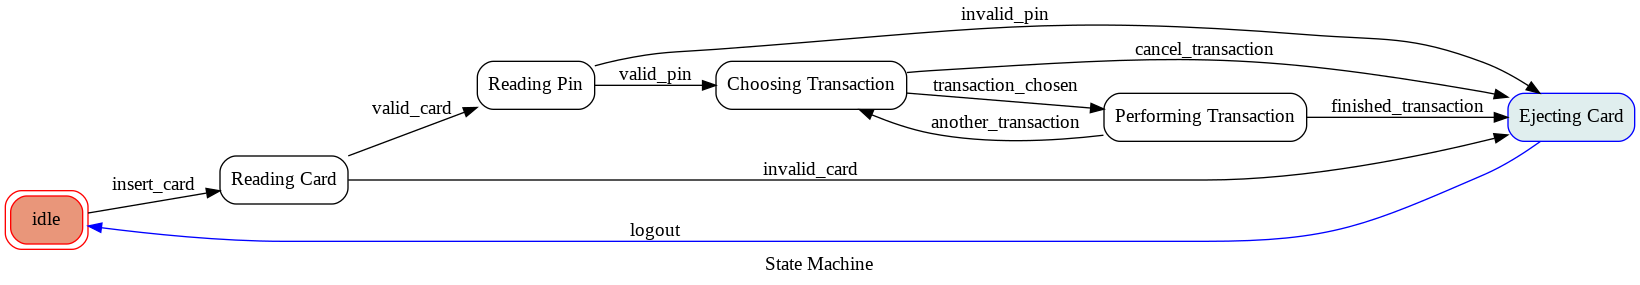
\includegraphics[width=1\textwidth,keepaspectratio]{images/FSM_ATM.png}
    \caption*{State Diagram of ATM created using graphviz}
\end{figure}

\subsubsection{Vending Machine as State Machine}
\normalsize{
The state machine of a vending machine was the final one I considered. The states that were available were "idle," "Count Coins," "Give Change," "Select Soda," and "Dispense Soda." The following commands were given as inputs: "insert coins," "reject coins," "cancel," "continue," and "shutdown." This time, in order to make it somewhat more challenging to understand, callbacks and conditions were included. The user has the option of selecting a beverage from the comprehensive selection that is provided. In addition, the user has the ability to input the amount of money that is placed into the vending machine, and the machine has the ability to accept or reject the coins depending on the quantity of money that it receives. Following the completion of the soda dispensing process, a "Thank You" message is shown to the user.
}
\begin{figure}[h!]
    \centering
    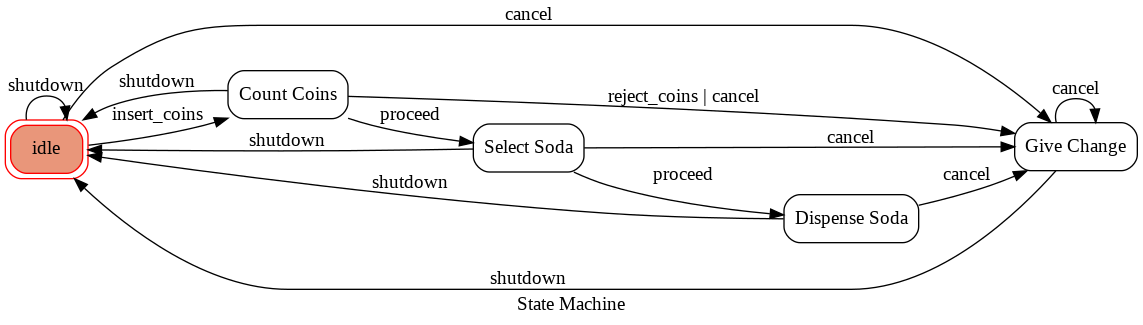
\includegraphics[width=\textwidth,keepaspectratio]{images/FSM_vending.png}
    \caption*{State Diagram of Vending Machine created using graphviz}
\end{figure}


\normalsize{
You may try some of the example FSMs created using pytransitions at the following Google Colab link : \url{https://colab.research.google.com/drive/1wyrW0FAUlreQRdu4wtCyQMBZo2KQ-x6P?usp=sharing}
}


\subsection{Angular}
\normalsize{
Angular is a web application framework that is built on TypeScript and is available for free and open source. It is managed by the Angular Team at Google as well as a community of people and organisations.\cite{angular}
As a platform, Angular includes:}
\begin{itemize}
    \item A component-based framework for building scalable web applications.
    \item A collection of well-integrated libraries that cover a wide variety of features, including routing, forms management and client-server communication.
    \item A suite of developer tools to help develop, build, test, and update the code.\cite{angular}
\end{itemize}

\normalsize{
The front-end development of the application is accomplished with the help of Angular.
}

\subsection{Django}
\normalsize{
Django is a free and open-source web framework written in Python that adheres to the model–template–views (MTV) architectural paradigm. It is maintained by the Django Software Foundation (DSF), an independent 501(c)(3) non-profit organisation formed in the United States.\cite{enwiki:1095293664}\\

The framework stresses component reusability and "pluggability," minimal code, low coupling, quick development, and the "don't repeat yourself" philosophy. Python is used everywhere, including settings, files, and data models. Django additionally has an alternate administration interface for create, read, update, and delete that is produced dynamically using introspection and set by admin models.\cite{enwiki:1095293664}\cite{django-docs}\\

Django is used for handling the back-end processes of the TreadWill application.
}

\subsection{Apache HTTP Server}
\normalsize{
Apache HTTP Server is a free, open-source, cross-platform web server application distributed under the Apache License 2.0. Under the aegis of the Apache Software Foundation, an open developer community creates and maintains Apache.\cite{enwiki:1100527453}\\

The great majority of Apache HTTP Server instances operate on a Linux distribution, although contemporary versions also run on Microsoft Windows, OpenVMS, and a number of Unix-like operating systems. Additionally, previous versions supported NetWare, OS/2, and other operating systems, as well as mainframe ports.\cite{enwiki:1100527453}\\

We configured the local Apache HTTP server to host the Angular-based front-end on custom network ports on an Ubuntu running PC.
}
\clearpage

\subsection{Daphne Server}
\normalsize{
Daphne is an HTTP, HTTP2, and WebSocket protocol server designed to enable Django Channels. It provides automated negotiation of protocols; URL prefixing is not required to distinguish between WebSocket and HTTP destinations.\cite{daphne} \\

Daphne is used in our project to host the Django-based back-end on custom network ports of the local system and handle requests from the front-end server (Apache). \\

To run a daphne server, we simply point Daphne to the ASGI application, and optionally set a bind address and port (defaults to localhost, port 8000):
\begin{verbatim}
    daphne myproject.asgi:application --port $PORT --bind $IP
\end{verbatim}
}
\begin{figure}[h!]
    \centering
    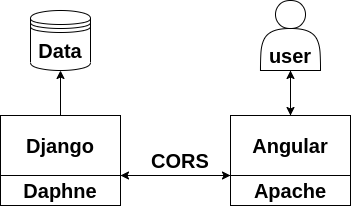
\includegraphics[width=0.7\textwidth,keepaspectratio]{images/workflow-treadwill.drawio.png}
    \caption*{Overview of our project}
\end{figure}
